\section{Design}\label{sec:design_clp}

\subsection{Common aspects}\label{subsec:common_aspects_clp}
Four different libraries have been realized:
\begin{itemize}
    \item \textbf{clp-core} for basic functionality of the other libraries
    \item \textbf{clpfd} for integer variables
    \item \textbf{clpqr} for rational and real variables
    \item \textbf{clpb} for boolean variables
\end{itemize}
\textbf{clpqr} contains basically the predicates of \textbf{clpq} and \textbf{clpr} of SWI Prolog because there
is any distinction between rational and reals in 2P-Kt.\newline
Libraries have been developed in this way to keep separated predicates which affect variables with different domains. This is useful because
each variabile type has own way to deal with constraints and searching for feasible solutions.
Libraries will be described in the following sections highlighting common and/or different aspects with respect to the SWI Prolog counterpart.

\subsection{Constraint Logic Programming over Finite Domains}\label{subsec:clpfd}
For a better explaination predicates will be divided in groups as described in section \ref{subsubsec:clp_libraries}.

\subsubsection{Arithmetic Constraints}\label{subsubsec:arithmetic_constraints}

All constraints supported by SWI Prolog are also supported in 2P-Kt; constraints are the followings:\newpage
\begin{center}
    \begin{table}
        \begin{tabular}{||c c ||} 
        \hline
        Constraint & Explaination \\ [0.5ex] 
        \hline\hline
        Expr1 \#= Expr2	& Expr1 equals Expr2 \\ 
        \hline
        Expr1 \#\= Expr2 & Expr1 is not equal to Expr2 \\
        \hline
        Expr1 \#>= Expr2 & Expr1 is greater than or equal to Expr2\\
        \hline
        Expr1 \#=< Expr2 & Expr1 is less than or equal to Expr2 \\
        \hline
        Expr1 \#> Expr2	& Expr1 is greater than Expr2 \\
        \hline
        Expr1 \#< Expr2	& Expr1 is less than Expr2 \\
        \hline
        \end{tabular}
        \label{table:arithmetic_constraints}
        \caption{Arithmetic constraints in clpfd}
    \end{table}    
\end{center}

\begin{center}
    \begin{table}
        \begin{tabular}{||c c ||} 
        \hline
        Expression & Explaination \\ [0.5ex] 
        \hline\hline
        integer	& Given value \\ 
        \hline
        variable & Unknown integer \\
        \hline
        -Expr & Unary minus\\
        \hline
        Expr + Expr	 & Addition \\
        \hline
        Expr * Expr	& Multiplication \\
        \hline
        Expr - Expr	& Subtraction \\
        \hline
        Expr \^ Expr& Exponentiation \\
        \hline
        min(Expr,Expr) & Minimum of two expressions \\
        \hline
        max(Expr,Expr) & Maximum of two expressions \\
        \hline
        Expr mod Expr & Modulo induced by floored division \\
        \hline
        abs(Expr) & Absolute value \\
        \hline
        Expr div Expr & Floored integer division \\
        \hline
        \end{tabular}
        \label{table:expressions_clp}
        \caption{Arithmetic expressions in clpfd}
    \end{table}    
\end{center}

\textit{Expr1} and \textit{Expr2} are \textbf{arithmetic expressions}.
\textit{Expr rem Expr} and \textit{Expr // Expr} are not supported. \textit{rem} is modulo induced by truncated division
whereas \textit{//} is truncated integer division.

\subsubsection{Membership Constraints}\label{subsubsec:Membership}

These constraints are used to specify the admissible domains of variables.\newline
The predicates are:\newline
\begin{itemize}
    \item \textbf{Var in Domain}: Var is an element of Domain; Domain is either an integer or an interval (expressed as Lower..Upper)
    \item \textbf{Vars in Domain}: The variables in the list Vars are elements of Domain
\end{itemize}

It is not current supported union of domains as expression for building a domain.

\subsubsection{Enumeration predicates}\label{subsubsec:enumeration}

These predicates are used to customize the search to find a feasible assignment of all variables such that all constraints are satisfied.\newline
The predicates are \textbf{labeling/2 and label/1}.\newline\newline
\textbf{labeling(Options, Vars)}\newline\newline
Assign a value to each variable in Vars; Options is a list of options that let exhibit some control over the search process. Several categories of options exist:
\begin{itemize}
    \item \textbf{variable selection strategy}: it can be the order in which the variable occurs (\textit{leftmost}, it is the default), the leftmost variable with smallest domain (\textit{ff}), the variables with smallest domains, the leftmost one participating in most constraints (\textit{ffc}), the leftmost variable whose lower bound is the lowest (\textit{min}) or the leftmost variable whose upper bound is the highest (\textit{max})
    \item \textbf{value order}: elements of the chosen variable's domain in ascending order (\textit{up}, it is the default) or domain elements in descending order (\textit{down})
    \item \textbf{branching strategy}: For each variable X, a choice is made between X = V and X \#\= V, where V is determined by the value ordering options. This option is called \textit{step}, it is the default and the only branching option supported
\end{itemize}

At most one option of each category can be specified, and an option must not occur repeatedly.\newline
The order of solutions can be influenced with:\newline
\begin{itemize}
    \item min(Expr)
    \item max(Expr)
\end{itemize}

This generates solutions in ascending/descending order with respect to the evaluation of the arithmetic expression Expr.\newline
The predicate \textbf{labeling/2} does not support as options the following branching strategies:\newline
\begin{itemize}
    \item \textit{enum}: For each variable X, a choice is made between X = V\_1, X = V\_2 etc., for all values V\_i of the domain of X. The order is determined by the value ordering options.
    \item \textit{bisect}: For each variable X, a choice is made between X \#=< M and X \#> M, where M is the midpoint of the domain of X.
\end{itemize}
\textbf{label(Vars)}\newline\newline
Equivalent to labeling([], Vars).

\subsubsection{Global constraints}\label{subsubsec:global_constraints}
A global constraint expresses a relation that involves many variables at once. The implemented constraints are the followings:
\begin{itemize}
    \item \textbf{all\_distinct(Vars)}: True iff Vars are pairwise distinct
    \item \textbf{sum(Vars, Rel, Expr)}: The sum of elements of the list Vars is in relation Rel to Expr. Rel is one of \#=, \#\=, \#<, \#>, \#=< or \#>=
    \item \textbf{scalar\_product(Cs, Vs, Rel, Expr)}: True iff the scalar product of Cs and Vs is in relation Rel to Expr. Cs is a list of integers, Vs is a list of variables and integers. Rel is \#=, \#\=, \#<, \#>, \#=< or \#>=
    \item \textbf{lex\_chain(Lists)}: Lists are lexicographically non-decreasing
    \item \textbf{tuples\_in(Tuples, Relation)}: True iff all Tuples are elements of Relation. Each element of the list Tuples is a list of integers or finite domain variables. Relation is a list of lists of integers
    \item \textbf{serialized(Starts, Durations)}: Describes a set of non-overlapping tasks. Starts = $[S_1,...,S_n]$, is a list of variables or integers, Durations = $[D_1,...,D_n]$ is a list of non-negative integers. Constrains Starts and Durations to denote a set of non-overlapping tasks, i.e.: S\_i + D\_i =< S\_j or S\_j + D\_j =< S\_i for all 1 =< i < j =< n
    \item \textbf{element(N, Vs, V)}: The N-th element of the list of finite domain variables Vs is V
    \item \textbf{global\_cardinality(Vs, Pairs)}: Global Cardinality constraint. Vs is a list of finite domain variables, Pairs is a list of Key-Num pairs, where Key is an integer and Num is a finite domain variable. The constraint holds iff each V in Vs is equal to some key, and for each Key-Num pair in Pairs, the number of occurrences of Key in Vs is Num
    \item \textbf{circuit(Vs)}: True iff the list Vs of finite domain variables induces a Hamiltonian circuit. The k-th element of Vs denotes the successor of node k
    \item \textbf{cumulative(Tasks, Options)}: Schedule with a limited resource. Tasks is a list of tasks, each of the form task(S\_i, D\_i, E\_i, C\_i, T\_i). S\_i denotes the start time, D\_i the positive duration, E\_i the end time, C\_i the non-negative resource consumption, and T\_i the task identifier. Each of these arguments must be a finite domain variable with bounded domain, or an integer. The constraint holds iff at each time slot during the start and end of each task, the total resource consumption of all tasks running at that time does not exceed the global resource limit. Options is a list of options. Currently, the only supported option is \textit{limit(L)} which is the global resource limit
    \item \textbf{cumulative(Tasks)}: Like the previous one but with \textit{L = 1}
    \item \textbf{disjoint2(Rectangles)}: True iff Rectangles are not overlapping. Rectangles is a list of terms of the form F(X\_i, W\_i, Y\_i, H\_i), where F is any functor, and the arguments are finite domain variables or integers that denote, respectively, the X coordinate, width, Y coordinate and height of each rectangle.
    \item \textbf{chain(Zs, Relation)}: Zs form a chain with respect to Relation. Zs is a list of finite domain variables that are a chain with respect to the partial order Relation, in the order they appear in the list. Relation must be \#=, \#=<, \#>=, \#< or \#>
\end{itemize}
\textbf{Notes}\newline\newline
Wrt global constraints provided by CLP(FD) library of SWI Prolog the following aspects are different:
\begin{itemize}
    \item the index of the predicate \textbf{circuit/1} starts from 1 and not from 0 for implementation issues
    \item the predicate \textbf{all\_different/1} has not been supported because it has the same usage of \textbf{all\_distinct} but it has a weaker propagation which cannot be simulated
    \item predicates \textbf{automaton/3} and \textbf{automaton/8} have not been implemented because of the fact that these predicates are rarely and difficult to use
    \item the predicate \textbf{global\_cardinality/3} can be used but actually it throws an exception because the Option parameter cannot be supported
\end{itemize}

\subsubsection{Reification Predicates}\label{subsubsec:reification}
All relational constraints discussed in \ref{subsubsec:arithmetic_constraints} can be reified.
This means that their truth value is itself turned into a clpfd variable, so that it is possible to reason about whether a constraint holds or not. These predicates are reifiable themselves.
\begin{itemize}
    \item \textbf{\#\ Q}: Q does not hold
    \item \textbf{P \#<==> Q}: P and Q are equivalent
    \item \textbf{P \#==> Q}: P implies Q
    \item \textbf{P \#<== Q}: Q implies P
    \item \textbf{P \#/\ Q}: P and Q hold
    \item \textbf{P \#\/ Q}: P or Q hold
    \item \textbf{P \#\ Q}: Either P holds or Q holds, but not both
    \item \textbf{zcompare(Order, A, B)}: reify an arithmetic comparison of two integers
\end{itemize}

\subsubsection{Reflection Predicates}\label{subsubsec:reflection}
Reflection predicates let obtain, in a well-defined way, information that is normally internal to this library. Predicates are:
\begin{itemize}
    \item \textbf{fd\_var(Var)}: True iff Var is a clpfd variable
    \item \textbf{fd\_inf(Var, Inf)}: Inf is the infimum of the current domain of Var
    \item \textbf{fd\_sup(Var, Sup)}: Sup is the supremum of the current domain of Var
    \item \textbf{fd\_size(Var, Size)}: Reflect the current size of a domain. Size is the number of elements of the current domain of Var
    \item \textbf{fd\_dom(Var, Dom)}: Dom is the current domain (see \ref{subsubsec:enumeration}) of Var
    \item \textbf{fd\_degree(Var, Degree)}: Degree is the number of constraints currently attached to Var
\end{itemize}

\subsection{Constraint Logic Programming over Rationals and Reals}\label{subsec:clpqr}
This library is very different from the previous one because variable definitions and constraints can be stated in the same predicate. The main predicate is
\textbf{\{\}(Constraints)} which allows to add the constraints given by Constraints to the constraint store.\newline
\textit{Constraints} can be defined using the following grammar:

\begin{figure}[h]
    \centering
    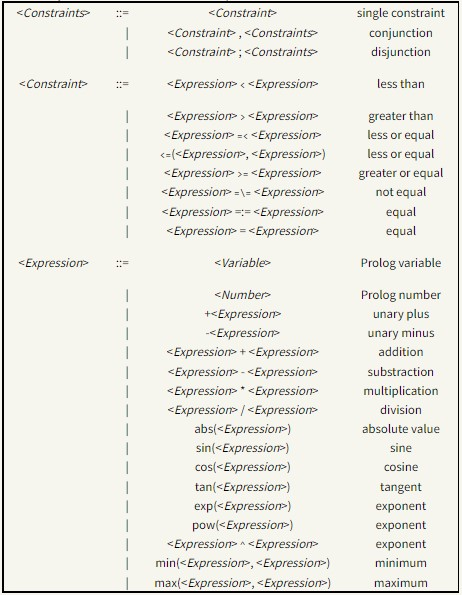
\includegraphics[width=0.70\textwidth]{images/bnf_constraints.jpg}
    \caption{clpqr constraints BNF}
    \label{fig:bnf_constraints}
\end{figure}

All constraints are supported except for \textit{<Expression> =\\= <Expression>} (not equal).
This libraries contains also the following predicates:
\begin{itemize}
    \item \textbf{satisfy(Vars)}: Provides for each variable in Vars a feasible assignment
    \item \textbf{entailed(Constraint)}: Succeeds if Constraint is necessarily true within the current constraint store. This means that adding the negation of the constraint to the store results in failure
    \item \textbf{inf(Expression, Inf)}: Computes the infimum of Expression within the current state of the constraint store and returns that infimum in Inf. This predicate does not change the constraint store
    \item \textbf{sup(Expression, Sup)}: Computes the supremum of Expression within the current state of the constraint store and returns that supremum in Sup. This predicate does not change the constraint store
    \item \textbf{minimize(Expression)}: Minimizes Expression within the current constraint store. This is the same as computing the infimum and equating the expression to that infimum
    \item \textbf{maximize(Expression)}: Maximizes Expression within the current constraint store. This is the same as computing the supremum and equating the expression to that supremum
    \item \textbf{bb\_inf(Ints, Expression, Inf, Vertex, Eps)}: It computes the infimum of Expression within the current constraint store, with the additional constraint that in that infimum, all variables in Ints have integral values. Vertex will contain the values of Ints in the infimum. Eps denotes how much a value may differ from an integer to be considered an integer
    \item \textbf{bb\_inf(Ints, Expression, Inf, Vertex)}: it behaves as the previous one but not use an error margin
    \item \textbf{bb\_inf(Ints, Expression, Inf)}: as the previous one but without returning the values of the integers
    \item \textbf{dump(Target, Newvars, CodedAnswer)}: Returns the constraints on Target in the list CodedAnswer where all variables of Target have been replaced by NewVars. This operation does not change the constraint store
\end{itemize}
\textbf{Notes}\newline\newline
Eps of the predicate \textbf{bb\_inf/5} cannot be fully supported, the only admissible value is 0.

\subsection{Constraint Logic Programming over Boolean Variables}\label{subsec:clpb}

All predicates of this library are based on the concept of \textit{boolean expression}. A \textit{boolean expression} is one of:
\begin{center}
    \begin{table}
        \begin{tabular}{||c c ||} 
        \hline
        Expression & Explaination \\ [0.5ex] 
        \hline\hline
        0 & false \\
        \hline
        1 & true \\ 
        \hline
        variable & unknown truth value \\
        \hline
        ~ Expr & logical NOT\\
        \hline
        Expr + Expr & logical OR \\
        \hline
        Expr * Expr & logical AND \\
        \hline
        Expr \# Expr & exclusive OR \\
        \hline
        Expr =:= Expr & equality \\
        \hline
        Expr =\= Expr & disequality (same as \#) \\
        \hline
        Expr =< Expr & less or equal (implication) \\
        \hline
        Expr >= Expr & greater or equal \\
        \hline
        Expr < Expr	& less than\\
        \hline
        Expr > Expr	& greater than \\
        \hline
        +(Exprs) & n-fold disjunction \\
        \hline
        *(Exprs) & n-fold conjunction \\
        \hline
        \end{tabular}
        \label{table:boolean_expressions}
        \caption{Admissible boolean expressions in clpb}
    \end{table}    
\end{center}

Supported predicates are:
\begin{itemize}
    \item \textbf{sat(Expr)}: True iff the Boolean expression Expr is satisfiable
    \item \textbf{taut(Expr, T)}: If Expr is a tautology with respect to the posted constraints, succeeds with T = 1. If Expr cannot be satisfied, succeeds with T = 0. Otherwise, it fails
    \item \textbf{labeling(Vs)}: Assigns truth values to the variables Vs such that all constraints are satisfied
    \item \textbf{sat\_count(Expr, Count)}: Count the number of admissible assignments. Count is the number of different assignments of truth values to the variables in the Boolean expression Expr, such that Expr is true and all posted constraints are satisfiable
    \item \textbf{weighted\_maximum(Weights, Vs, Maximum)}: Enumerate weighted optima over admissible assignments. Maximize a linear objective function over Boolean variables Vs with integer coefficients Weights. This predicate assigns 0 and 1 to the variables in Vs such that all stated constraints are satisfied, and Maximum is the maximum of $sum(Weight_i*V_i)$ over all admissible assignments
    \item \textbf{random\_labeling(Seed, Vs)}: Select a single random solution. An admissible assignment of truth values to the Boolean variables in Vs is chosen in such a way that each admissible assignment is equally likely. Seed is an integer, used as the initial seed for the random number generator
\end{itemize}


